\documentclass{scrbook}

\KOMAoptions{%
    fontsize=10pt,          % Tamaño de fuente
    paper=a4,               % Tamaño del papel
    headings=normal,        % Tamaño de letra para los títulos: small, normal,
                            % big
    parskip=full,           % Espacio entre párrafos: full (una línea) o half
                            % (media línea)
    headsepline=false,      % Una linea separa la cabecera del texto
    cleardoublepage=empty,  % No imprime cabecera ni pie en páginas en blanco 
    chapterprefix=false,    % No antepone el texto "Capítulo" antes del número
    appendixprefix=false,	% No antepone el texto "Apéndice" antes de la letra
    listof=totoc,		    % Añade a la tabla de contenidos la lista de tablas 
                            % y figuras
    index=totoc,			% Añade a la talba de contenidos una entrada para 
                            % el índice
    bibliography=totoc,	    % Añade a la tabla de contenidos una entrada para
                            % bibliografía
    BCOR=5mm,               % Reserva margen interior para la encuadernación. 
                            % El valor dependerá el tipo de encuadernado y del
                            % grosor del libro.
    DIV=10,                 % Cálcula el diseño de página según ciertos 
                            % parámetros. Al aumentar el número aumentamos el
                            % ancho de texto y disminuimos el ancho del margen.
                            % Una opción de 14 producirá márgenes estrechos y
                            % texto ancho.
}

% Set input encoding.
\usepackage[utf8]{inputenc}

% Establish Spanish as the default language. English is also used in the
% abstract.
%   es-tabla - Change "Cuadro" for "Tabla".
\usepackage[english, spanish, es-tabla]{babel}

% Set graphics folder path.
\usepackage{graphicx}
\graphicspath{{images/}}

% Enable graphics placement.
\usepackage{float}

% Apply color to tables.
\usepackage{colortbl}

% Set title page background image.
\usepackage{eso-pic}
\newcommand\BackgroundPic{%
	\put(0,0){%
		\parbox[b][\paperheight]{\paperwidth}{%
			\vfill
			\centering
			
\includegraphics[width=\paperwidth,height=\paperheight,%
			keepaspectratio]{ugr/portada-sencilla-color}%
			\vfill
}}}

% Add the euro symbol.
\usepackage{marvosym}
\DeclareUnicodeCharacter{20AC}{\EUR{}}

\usepackage{hyperref}
\usepackage{booktabs}
\usepackage{bookmark}

% Change second level label item to a dash.
\renewcommand{\labelitemii}{--}

\begin{document}

\frontmatter
\begin{titlepage}
    \AddToShipoutPicture*{\BackgroundPic}

    \begin{addmargin}[2.575cm]{0cm}
        \begin{flushleft}
            \Large
            \hfill\vfil

            \large{\textsf{Escuela Técnica Superior en Ingenierías Informática y de Telecomunicación}}
            \vfill

            {\large\textsc{Máster Universitario en Ingeniería Informática}} \vfill


            {\large\textsc{trabajo de fin de máster}}

            \begingroup
            \Huge{Título del TFM}
            \endgroup

            \vfill\vfill\vfill\vfill

            \textsf{\normalsize{Presentado por:}}\\
            {\normalsize\textrm{Víctor Vázquez Rodríguez}}
            \bigskip

            \textsf{\normalsize{Tutor:}}\\
            {\normalsize\rmfamily{
                Antonio Javier Díaz Alonso\\
                \emph{Departamento de Arquitectura y Tecnología de Computadores}
            }}

            \bigskip
            \textsf{\normalsize{Curso académico 2020-2021}}
        \end{flushleft}
    \end{addmargin}
\end{titlepage}
\cleardoublepage
\pdfbookmark[1]{Agradecimientos}{Agradecimientos}

\chapter*{Agradecimientos}

Al Dr. Antonio Javier Díaz Alonso, tutor de este trabajo, por guiarme y
aportarme su experiencia académica.

A mis padres, por darme la oportunidad de estudiar y seguir mi propio camino.

Al Dr. Juan Antonio Vázquez Rodríguez, mi hermano, por ser mi referente de
esfuerzo, trabajo, bondad y humildad.

A mi novia, Rosa, por creer siempre en mí y estar a mi lado pase lo que pase.

A mis compañeros de promoción del Máster, por hacerme sentir como en casa lejos
de ella.

\cleardoublepage
\pdfbookmark[1]{Resumen}{Resumen}

\chapter*{Resumen}

\selectlanguage{spanish}
Con el advenimiento de la Industria 4.0, las empresas buscan incorporar técnicas
de inteligencia artificial y análisis de datos a sus instalaciones y procesos
industriales con el objetivo de mejorar la productividad y la autonomía. En este
trabajo, se plantea la posibilidad de usar tecnologías de contenerización de
procesos para el despliegue eficiente de estas nuevas tareas junto con las de
tiempo real habituales en los sistemas de control industrial, estudiando las
distintas tecnologías posibles y realizando un análisis del rendimiento de
tareas de tiempo real contenerizadas con Docker. Además, se diseña e implementa
una herramienta software que sirve como prueba de concepto para el despliegue y
la orquestación de este tipo de tareas sobre entornos distribuidos mediante el
uso de contenedores.

\selectlanguage{english}
\itshape
As Industry 4.0 gets closer, companies are looking to incorporate artificial
intelligence and data analysis techniques to their facilities and industrial
processes with the objective of improving productivity and autonomy. This paper
proposes the use of processes containerization techonologies for efficient
deployment of these new tasks along with the real-time tasks that are common in
industrial control systems, studying different possible techonologies and
analysing the performance of real-time tasks containerized using Docker.
Finally, a proof-of-concept software tool for deployment and orchestration of
this type of tasks on distributed environments by means of containers.

\selectlanguage{spanish}

\cleardoublepage
\pdfbookmark[1]{\contentsname}{toc}

\tableofcontents
\listoffigures
\listoftables
\lstlistoflistings

\cleardoublepage

\mainmatter
\chapter{Introducción}

\section{Motivación y contexto}

El Programma 101 es considerado por muchos como el primer ordenador de uso
personal. Producido por la empresa italiana Olivetti entre los años 1962 y 1964,
este dispositivos seasimilaba más a una calculadora que al concepto de ordenador
que se tiene en la actualidad. Casi 60 años después, los ordenadores han
evolucionado hasta convertirse en un objeto asequible y casi indispensable,
teniendo la mayor parte de la sociedad acceso a algún dispositivo con capacidad
de computación. Aspectos de nuestra vida como el ocio, serían muy diferentes sin
las redes sociales o los servicios online. Esta evolución de los ordenadores y
la computación en general continúa hoy en día, buscando conectar dispositivos
cotidianos a internet e incorporar en ellos cierta capacidad de procesamiento.
Televisores inteligentes en los que instalar aplicaciones, robots aspiradores
que funcionan de manera autónoma, frigoríficos que permiten ver el estado de los
alimentos que almacenan, todos estos productos surgen de la expansión de los
ordenadores hasta todos los rincones de nuestras vidas, con el objetivo final de
hacerla más sencilla para los humanos. Esta expansión no está ocurriendo solo en
los hogares, si no que se avanza hacia un mundo más conectado donde
aparentemente todo lo que nos rodea tenga acceso a la red.

La industria no es ajena a este cambio, ya que la aplicación del internet de las
cosas (IoT por sus siglas en inglés) a los procesos industriales podría aportar
beneficios muy importantes como son el aumento de la productividad, de la
calidad de los productos o de la seguridad de las instalaciones. No obstante, se
trata de un proceso de implantación complejo y de muy largo plazo, debido a los
estrictos requisitos de algunos sectores industriales. Las fábricas y plantas de
producción relegan las tareas de control de sus operaciones a los sistemas de
control industriales o ICSs (\textit{Industrial Control Systems}). Normalmente,
estos sistemas deben responder ante eventos que ocurren en las instalaciones en
ventanas de tiempo muy pequeñas, dependiendo del proceso concreto y sus riesgos
asociados. La fiabilidad de estos sistemas y su tolerancia ante los fallos es de
gran importancia, siendo crucial la verificación de estos aspectos durante su
diseño y desarrollo. Es por estos requisitos tan estrictos que, en muchos casos,
para la implantación de los ICSs se utilizan tanto \textit{hardware} como
\textit{software} específicos y que ya han sido validados para este tipo de
aplicaciones. No obstante, el uso de estas herramientas también plantea algunos
inconvenientes, como por ejemplo la difícil interoperabilidad con otros sistemas
debido a la naturaleza cerrada de las mismas o la reutilización del código en
otras plataformas, lo que acorta la vida útil del \textit{software}.

Desde esta situación se afronta el avance hacia la cuarta revolución industrial
o Industria 4.0. Uno de los objetivos principales que se persigue es la
automatización completa de los procesos industriales, haciando que sean
independientes y autogestionados, aumentando así su eficiencia, productividad y
seguridad. Para conseguir este objetivo, es necesario incorporar a estos
procesos las nuevas técnicas de aprendizaje automático y análisis de grandes
volúmenes de datos, construyendo sistemas experots capaces de tomar decisiones
propias para su funcionamiento y gestión (p. ej., modificar el ritmo de
producción en base a predicciones sobre la demanda). Aunque estos sistemas
expertos se podrían desplegar en plataformas separadas de las que habitan los
ICSs, esto duplica los costes de infraestructura y hace también más difícil el
mantenimiento de la misma. Por ello, hay una tendencia cada vez mayor hacia la
ejecución de tareas con distintos niveles de criticalidad en una misma
plataforma. Por otra parte, las tareas de aprendizaje máquina suelen requerir de
una capacidad de computación relativamente elevada, sobre todo cuando la
cantidad de datos sobre la que se trabaja es grande. Un solo dispositivo no
sería capaz de gestionar estas tareas de forma eficiente si, además, debe
realizar tareas críticas de control, dificultando también que pueda cumplir con
sus requisitos en ese aspecto. Aparecen entonces nuevos paradigmas de
computación, como el \textit{fog} o el \textit{edge computing}, que pretenden
decentralizar el procesamiento, alejándolo de la nube y llevándolo a elementos
intermedios más cercanos a las fuentes de datos o a los dispositivos del borde
de la red, respectivamente. En estos paradigmas, se persigue la máxima
utilización de la capacidad de computación de los dispositivos presentes en la
red, distribuyendo entre ellos las tareas necesarias de forma dinámica.

Dentro de este campo, se están llevando a cabo muchas investigaciones para
validar la efectividad de estos nuevos modelos y hacerlos realidad, además de
comprobar su efectividad en el ámbito industrial. Uno de los planteamientos más
prometedores es el que conlleva la aplicación de tecnologías de virtualización a
los sistemas de control industrial, permitiendo su despliegue y ejecución
distribuida en convivencia con otros procesos. Estas tecnologías, que han
sufrido un desarrollo masico en los últimos años debido al auge de la
computación en la nube, pueden ahora ser claves para asegurar la resiliencia y
robustez de los ICSs en entornos distribuidos.

Por todo esto, este trabajo abordará la complejidad de los problemas descritos
intentando buscar mecanismos que simplifiquen la gestión de los sistemas
\textit{fog}/\textit{edge}. Partiremos de la experiencia previa en trabajos con
contenedores orientados al análisis de sus prestaciones para la ejecución de
tareas con restricciones temporales, responsables de las ideas aquí propuestas y
base fundamental de parte de la motivación de este trabajo. Además, esta línea
de investigación tiene mucho potencial para mejorar los sistemas de control
implementados en la actualidad, permitiendo por tanto una contribución
importante tanto en aspectos industriales como científicos, lo que aumenta aún
más nuestro interés en esta temática.

\section{Objetivos}

De cara a la realización de este trabajo, se han planteado los siguientes
objetivos a cumplir:

\begin{itemize}
    \item Comprender los conceptos básicos sobre sistemas operativos de tiempo
          real, algoritmos de planificación y sistemas de control industriales.
    \item Analizar las soluciones de tiempo real basadas en GNU/Linux existentes.
    \item Estudiar la viabilidad y rendimiento de las tecnologías de
          contenerización para la ejecución de tareas con restricciones temporales.
    \item Diseñar e implementar una herramienta de despliegue de tareas de
          tiempo real mediante contenedores que sirva como prueba de concepto.
    \item Caracterizar las prestaciones de la herramienta desarrollada,
          identificando posibles aplicaciones y/o mejoras de la misma.
\end{itemize}

Una parte relevante de los objetivos del presente proyecto están asociados al
estudio y caracterización de tecnologías, así como al análisis del mercado, que
se justifica por un enfoque innovador orientado al desarrollo de sistemas para
\textit{fog computing}. Esto, junto con los conocimientos adquiridos sobre
implementación de sistemas de tiempo real, será clave para que la herramienta
desarrollada como prueba de concepto sea lo más eficiente y funcional posible.

Por otra parte, en los objetivos también se hace hincapié en el uso de
soluciones basadas en GNU/Linux, como parte de un fuerte compromiso con las
herramientas libres y de código abierto. Algunos de los sistemas operativos de
tiempo real más conocidos y usados son de código propietario y es necesario
adquirir licencias para utilizarlos, lo cual no favorece ni el aprendizaje ni la
reutilización del software desarrollado para estas plataformas. Últimamente, se
han realizado contribuciones importantes al kernel de Linux para mejorar el
soporte que ofrece a cargas de trabajo de este tipo, además de los múltiples
proyectos más especializados que está llevando a cabo la comunidad. En esta
aproximación, hemos considerado primordial la extensión del software libre,
apoyando su uso siempre que sea posible. Por ello, la herramienta planteada se
diseñará en torno al despliegue de tareas en sistemas GNU/Linux.

\section{Planificación}

\section{Material y métodos}

En esta sección, se presentan todas las herramientas que se han usado para
llevar a cabo este proyecto, además de las metodologías de trabajo seguidas. En
la figura \ref{fig:01-tools} se puede ver una recopilación de los logotipos de
todas estas herramientas, las cuales se van a exponer en detalle a continuación.

En un proyecto de desarrollo de código como es este, una de las herramientas más
importantes es la de control de versiones. En nuestro caso, se ha usado
\textbf{Git} debido a que es una herramienta de código libre y, además, es la
más conocida y usada. El repositorio remoto se ha alojado en \textbf{GitHub}, la
popular plataforma de desarrollo de código colaborativo. El desarrollo de código
como tal se ha hecho con \textbf{Visual Studio Code}, un editor de texto de
Microsoft que, aunque ofrece menos funcionalidad de serie que los entornos de
desarrollo (IDEs) especializados, también es mucho más liviano y rápido. Además,
esta funcionalidad se puede extender enormemente mediante extensiones, pudiendo
convertirlo casi en un IDE adaptado a las necesidades concretas del usuario.
Gracias a estas extensiones, se puede usar el mismo editor para distintos
programar en distintos lenguajes, lo cual ha sido una de las principales razones
por las que se ha escogido.

Como ya se ha indicado en la sección anterior, se ha aplicado un SCRUM adaptado
como metodología de planificación, gestión y seguimiento del proyecto, usando un
tablero Kanban para la visualización de las tareas. Concretamente, se ha usado
el tablero que ofrece GitHub como parte de sus herramientas para la gestión de
proyectos. Las tareas se añaden a los repositorios como \textit{issues}, los
cuales se añaden al tablero para controlar su estado de realización. El
beneficio que nos aporta el uso de GitHub para esto es el de tener una
plataforma unificada tanto para la gestión del proyecto como para su desarrollo.
Esta integración permite flujos de trabajo muy interesantes, como por ejemplo
referenciar los \textit{issues} ya mencionados en los mensajes de
\textit{commit}, de forma que se vinculan los cambios realizados con la tarea en
la que se engloban. La gestión del proyecto es, por tanto, más directa y
sencilla.

\textbf{Incorporar imagen del tablero del proyecto de GitHub}

Los diagramas que se presentan a lo largo de este trabajo, incluidos los que
componen el diseño de la herramienta desarrollada y sus componentes, se han
creado con la herramienta online \textbf{draw.io}. Al integrarse directamente
con Google Drive, se puede usar desde el navegador, siendo una solución muy
cómoda y accesible para la creación de estos diagramas.

En cuanto al desarrollo y despliegue de la herramienta planteada, se han
utilizado varias tecnologías. Los lenguajes de programación son Python y C, muy
conocidos y utilizados en la industria. C es el lenguaje de referencia para la
programación de sistemas y las tareas de bajo nivel, mientras que Python ofrece
una sintaxis muy sencilla para la implementación de herramientas como
aplicaciones o servidores. Python también posee una nutrida colección de
librerías para distintos casos de uso, lo cual también fue muy atractivo para su
elección. En este proyecto, se usan varias de estas librerías para facilitar la
implementación de algunos aspectos de la herramienta. Destacamos las siguientes:

\begin{itemize}
    \item \textbf{hug} - Escritura de APIs sencilla y sin ataduras. Esta
          librería trata de competir con otras más conocidas como Flask, proponiendo
          un modelo mucho más simple y dando más libertad al desarrollador.
    \item \textbf{click} - Más que una librería, se trata de un
          \textit{framework} para la implementación de aplicaciones de línea de
          comandos (CLI). Ofrece todas las utilidades que se pueden necesitar para
          este tipo de aplicaciones, como es la generación automática de páginas de
          ayuda.
    \item \textbf{marshmallow} - Esta librería permite la sencilla
          deserialización y serialización de objetos JSON a objetos Python. Esto es
          especialmente útil al trabajar con servicios web, ya que se pueden leer los
          datos JSON recibidos y validarlos frente a un esquema de datos definido por
          el desarrollador.
    \item \textbf{pymongo} - Ejecución de consultas sobre bases de datos
          MongoDB, que son las usadas en este proyecto.
    \item \textbf{paramiko} - Herramientas para trabajar con SSH desde Python.
          Esencial para el despliegue de las tareas sobre los nodos.
    \item \textbf{docker} - La librería oficial de Docker para Python. Con ella,
          se puede conectar con un servidor Docker (local o remoto) para ejecutar
          operaciones de construcción de imágenes o lanzamiento de contenedores.
    \item \textbf{requests} - Es la librería más conocida para la realización de
          peticiones HTTP en Python.
    \item \textbf{unittest} - Aunque no se trata de una librería externa como
          las demás, ya que forma parte de la librería estándar de Python, merece ser
          destacada por ser la utilizada para la escritura y ejecución de las pruebas
          del código desarrollado.
\end{itemize}

Además de estas librerías, se han usado otras para el análisis y formateo del
código como son \textbf{pylint} y \textbf{autopep8}.

Como ya se ha mencionado, la herramienta desarrollada trabaja con
\textbf{MongoDB} para la gestión del almacenamiento persistente de los datos y
el acceso a los mismos. Se trata de un gestor de bases de datos documental que
pertenece a la familia NoSQL (\textit{Not only SQL}). Las bases de datos
documentales divergen del modelo relacional tradicional que siguen otros
gestores tan famosos como MySQL o PostgreSQL. No existen los conceptos de tabla
o fila, sino que se almacenan colecciones de documentos no estructurados. En el
caso de MongoDB, se trabaja con documentos JSON, formato ampliamente usado en el
entorno web para la transmisión de datos debido a su legibilidad y velocidad de
serialización/deserialización. Cuando decimos que los documentos son no
estructurados, nos referimos a que no tienen por qué poseer los mismos campos,
ya que no hay un esquema definido a seguir. MongoDB no cumple con ACID, pero es
una pérdida aceptable a cambio de la flexibilidad y facilidad de uso que nos
ofrece. Además, el lenguaje de consultas es mucho más claro e intuitivo que SQL,
permitiendo realizar consultas de envergadura similar.

\begin{figure}[H]
    \centering
    
\includegraphics[width=0.7\textwidth]{01-introduction/tools.png}
    \caption{Logotipos de las herramientas utilizadas. De izquierda a derecha y%
        de arriba a abajo: Python, Docker, Raspberry Pi, GitHub, VS Code y
        draw.io}
    \label{fig:01-tools}
\end{figure}

La idea principal en torno a la cual gira este trabajo es la del uso de
contenedores para el despliegue de tareas de tiempo real. En este sentido,
\textbf{Docker} es la tecnología de contenerización en la que nos hemos apoyado
para la implementación de la herramienta propuesta. Esta elección recae
principalmente en el hecho de que se trata del motor de contenedores más
conocido y utilizado. De la mano de Docker, también se ha utlizado
\textbf{Docker Compose} para el despliegue sencillo de un entorno de desarrollo
completo que permita replicar un despliegue de producción de forma simplificada.
Las imágenes de contenedores definidas en este proyecto, se han alojado en el
repositorio de imágenes \textbf{DockerHub}, aprovechando que proporciona un
sistema de construcción automática de imágenes.

Para realizar las pruebas del sistema desarrollado, se ha usado una
\textbf{Raspberry Pi 4B}, concretamente la que se muestra en la figura
\ref{fig:01-raspberry-pi}. Se trata de un SBC (\textit{Single Board Computer})
de bajo coste y muy versátil, pudiendo usarse para infinidad de aplicaciones.
Las características detalladas de esta plataforma se pueden ver en la tabla \ref{tab:01-raspberry-specs}.

\begin{table}[H]
    \centering
    \begin{tabular}{ |>{\columncolor[gray]{0.8}}l|p{0.5\textwidth}| }
        \hline
        \textbf{Procesador}          & Cortex-A72                \\
        \hline
        \textbf{Arquitectura}        & ARMv7                     \\
        \hline
        \textbf{Número de núcleos}   & 4                         \\
        \hline
        \textbf{Frecuencia de reloj} & 1500 MHz                  \\
        \hline
        \textbf{RAM}                 & 4 GB                      \\
        \hline
        \textbf{Sistema operativo}   & Raspberry Pi OS Lite 4.19 \\
        \hline
    \end{tabular}
    \caption{Especificaciones de la Raspberry Pi usada en el trabajo}
    \label{tab:01-raspberry-specs}
\end{table}

El sistema operativo de este dispositivo es GNU/Linux (concretamente, basado en
Debian), y se le ha aplicado la revisión 24 del parche de tiempo real
\textbf{PREEMPT-RT}. Este parche aporta al sistema la capacidad de realizar
planificación de procesos apropiativa.

\begin{figure}
    \centering
    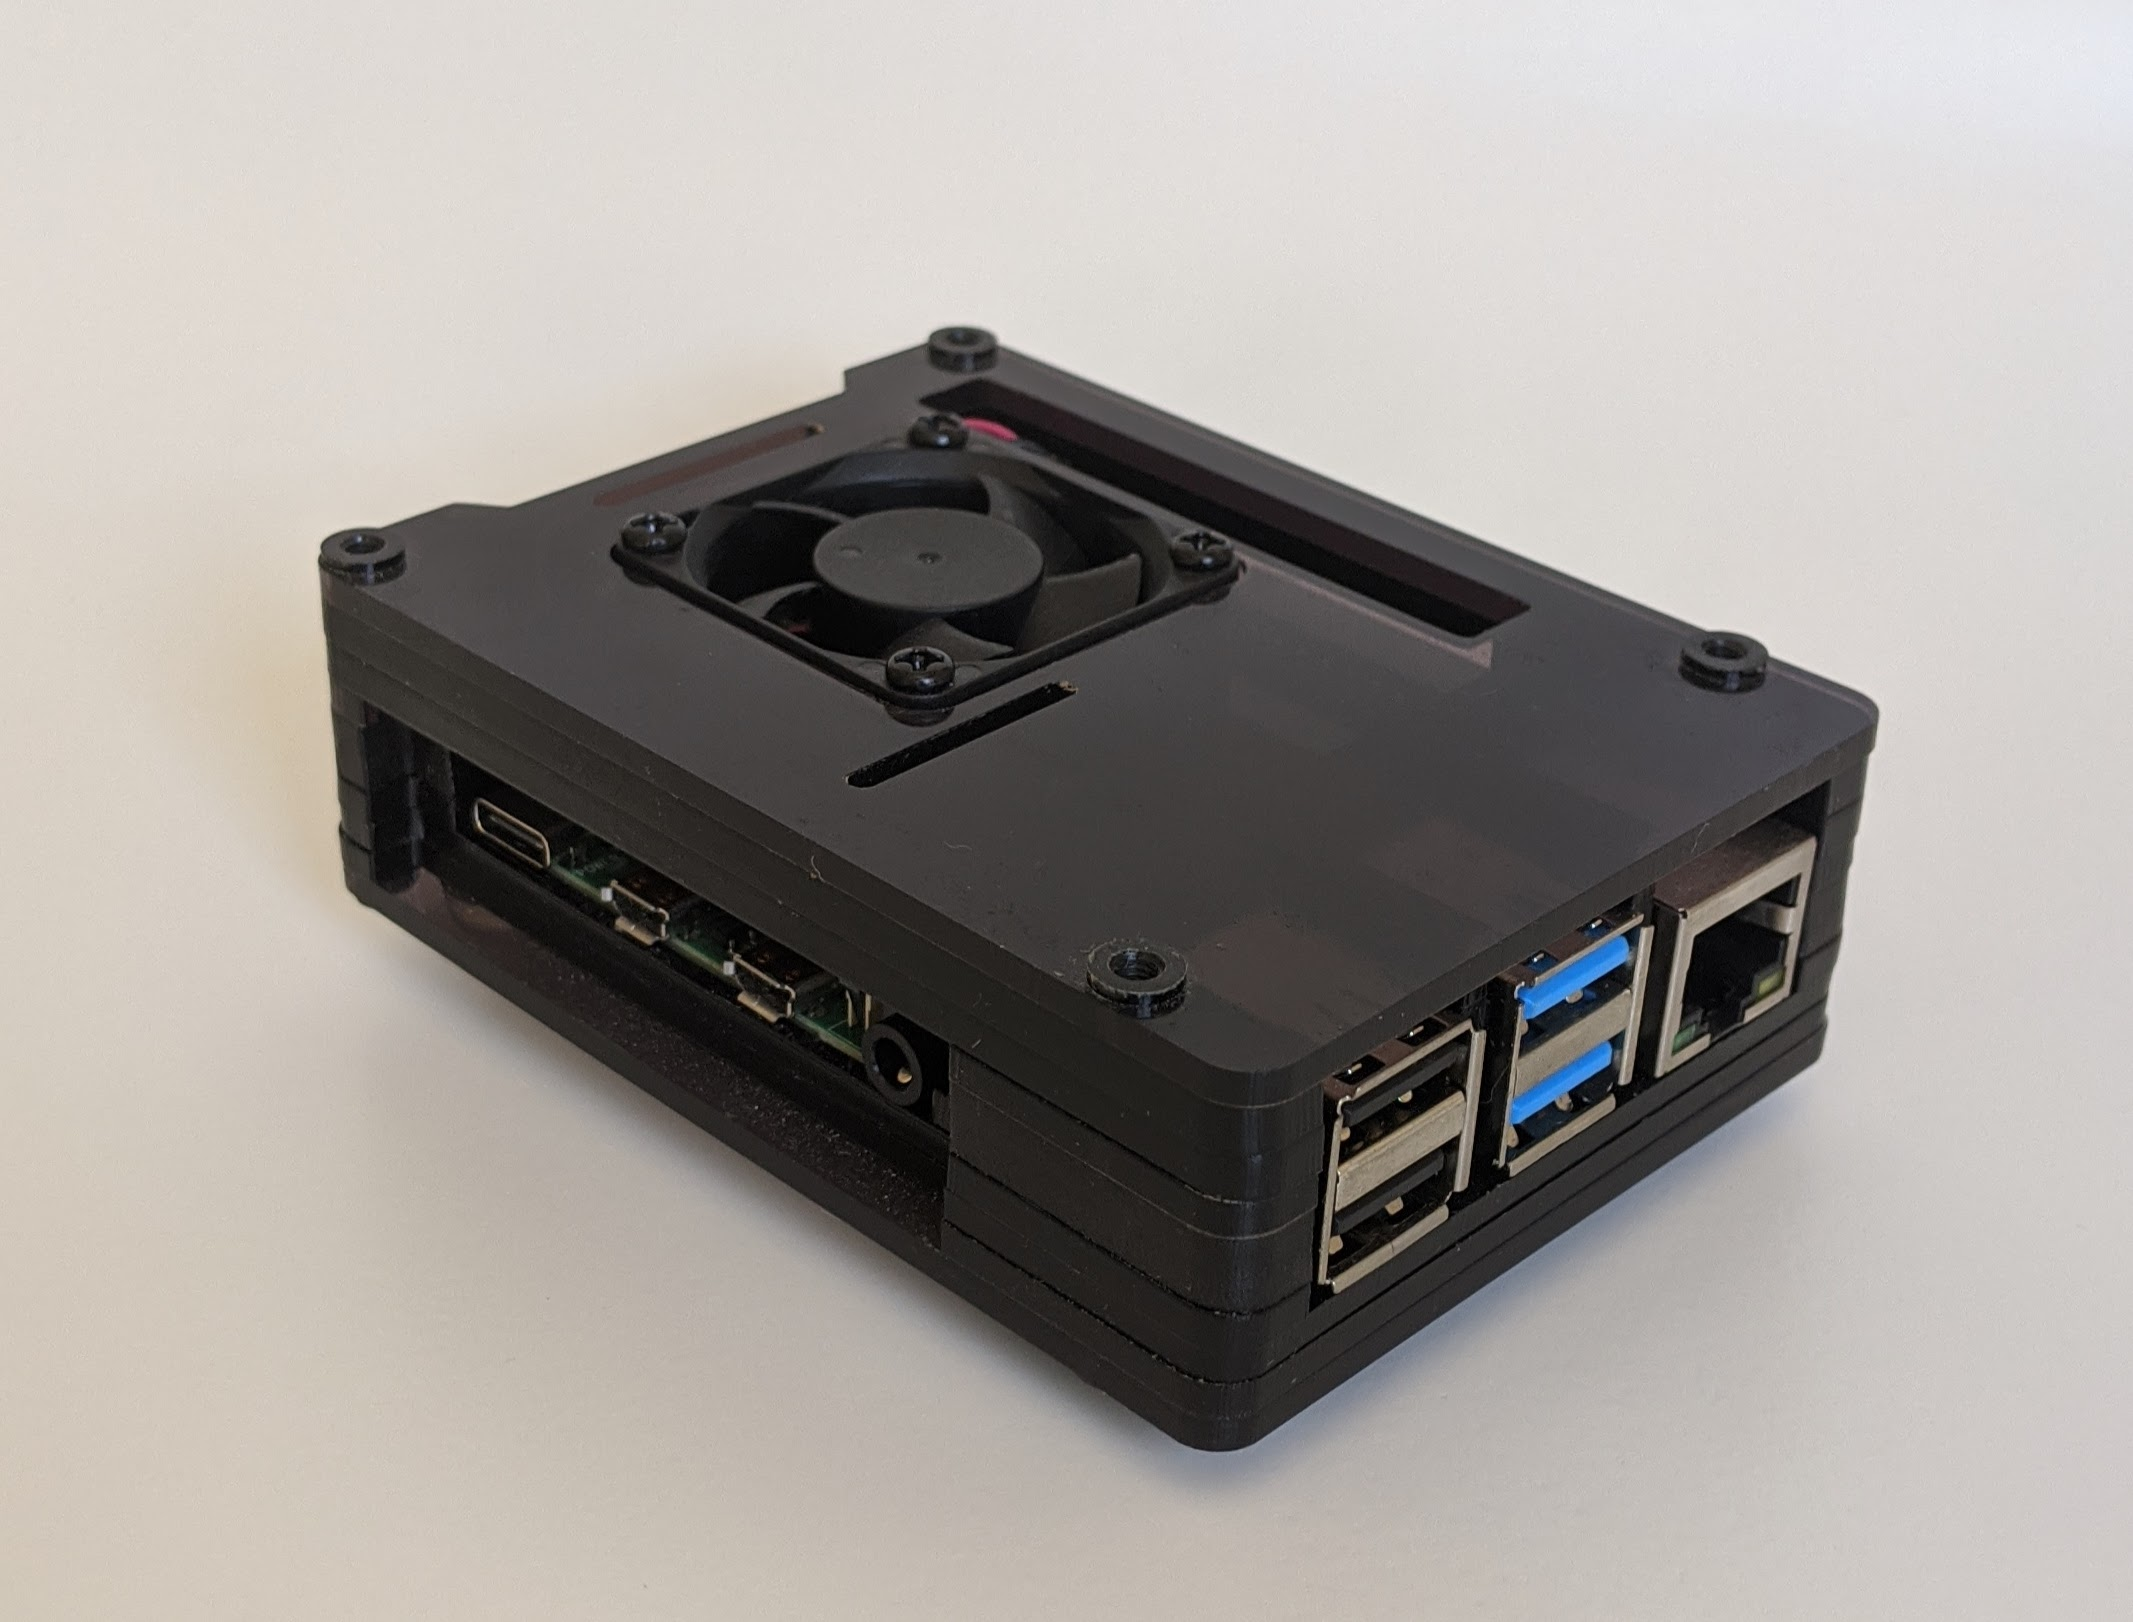
\includegraphics[width=0.8\textwidth]{01-introduction/raspberry-pi.jpg}
    \caption{Raspberry Pi 4B utilizada en el trabajo}
    \label{fig:01-raspberry-pi}
\end{figure}

\section{Estructura de la memoria}

La estructura de la presente memoria es la siguiente:

En el capítulo 1, se ha introducido el proyecto y explicado tanto la motivación
detrás del mismo como los objetivos planteados, la planificación seguida y las
herramientas, tecnologías y metodologías que se han utilizado.

En el capítulo 2, se realiza un estudio en profundidad del estado de la técnica
en lo relativo a los sistemas confiables, las tareas de tiempo real y las
tecnologías de virtualización. Se presentan otros estudios interesantes llevados
a cabo en esta área y se introducen todos los conceptos relevantes.

En la sección 3, se aborda el diseño de una herramienta para el despliegue y
seguimiento de tareas de tiempo real en entornos distribuidos, así como su
implementación y prueba. Se presentan los resultados obtenidos y se discute
sobre los mismos.

En la sección 4, se realiza una revisión del proyecto completo y se presentan
las conclusiones, así como las maneras en las que se puede extender y mejorar el
trabajo realizado.

\chapter{Revisión del estado de la técnica}

Antes de poder aventurarnos el desarrollo de una herramienta para la
orquestación de tareas de tiempo real usando contenedores, es necesario
estudiar y comprender los fundamentos y peculiaridades de diversos campos como
son los sistemas de tiempo real, la planificación de procesos, la computación en
la nube o las tecnologías de virtualización. En este capítulo, se introducen los
conceptos más importantes de estos campos, además de revisar otros trabajos
realizados con el objetivo de comprobar cuál es el estado de la investigación
en dichos temas.

\section{Sistemas empotrados, confiables y de criticalidad mixta}

Los ordenadores y teléfonos inteligentes que usamos a diario nos permiten
realizar multitud de tareas diferentes: desde leer el correo o navegar por
internet hasta editar imágenes y vídeos o realizar videollamadas. Aunque no nos
demos cuenta, interactuamos habitualmente con muchos más sistemas informáticos
además de los ya mencionados. La computación está presente en los coches, los
trenes, los aviones, los satélites espaciales, los televisores o las lavadoras.
Estos sistemas, que reciben el nombre de sistemas empotrados, son diseñados para
llevar a cabo de manera óptima un conjunto de tareas específico, frente al
enfoque generalista de los ordenadores de uso personal. Como se introduce en
\cite{wolf_high-performance_2014}, los sistemas empotrados son comunes en
contextos en los que el rendimiento es primordial, como son las comunicaciones
de red o la compresión/decompresión de audio y vídeo para retransmisiones en
directo. En este libro se exponen diversas aplicaciones de los sistemas
empotrados de alto rendimiento para sistemas ciber-físicos o CPS
(\textit{Cyber-Physical Systems}). Los CPS son, en esencia, sistemas
informáticos que interactúan con procesos físicos, actuando en función de los
cambios en su entorno. Este aspecto hace que el diseño y la implementación de
los CPS difiera considerablemente del resto de sistemas empotrados, ya que hay
que prestar especial atención a las características del entorno en el que se
desplegará el sistema y a los mecanismos de entrada y salida (interacción con el
entorno), además de optimizar el consumo de memoria y procesamiento para cumplir
con las limitaciones del hardware \cite{lee_introduction_2016}.

En algunos casos, estos sistemas son críticos, lo que significa que un fallo en
su funcionamiento supone daños graves a las personas o al medio ambiente. Este
es el caso de los aviones, los trenes o las plantas nucleares, por ejemplo. En
estos sistemas, cobra especial importancia el concepto de confiabilidad, es
decir, garantizar el correcto funcionamiento del sistema en todo momento. En la
figura \ref{fig:01-dependability} se pueden apreciar los atributos que debe
poseer un sistema confiable. A nivel de software, existen arquitecturas y
patrones de diseño orientados a garantizar la tolerancia ante los fallos del
mismo \cite{pullum_software_2001}\cite{randell_system_1975}. Por otra parte, la
replicación de componentes \cite{hutchison_dependable_2006} es una técnica muy
usada tanto para el software como el hardware. Lo que se intenta con la
replicación es asegurar que un cálculo o procesamiento se lleva a cabo de forma
correcta, aunque alguna de las réplicas falle. En \cite{amin_review_2019}, se
realiza una revisión de los sistemas de control tolerantes ante fallos
dividiéndolos en tres tipos: AFTCS (\textit{Active Fault Tolerant Control
  Systems}), PFTCS (\textit{Passive Fault Tolerant Control Systems}) o HFTCS
(\textit{Hybrid Fault Tolerant Control Systems}). Para cada uno de estos tipos,
los autores presentan las principales arquitecturas usadas, los modelos de
análisis matemático usados para su validación y las últimas técnicas usadas para
su diseño. Por otra parte, el estudio realizado en \cite{shan_survey_2019} tiene
como objetivo analizar la aplicación de los estándares de seguridad, protección
y privacidad al diseño y desarrollo de sistemas confiables, llegando los autores
a la conclusión de que cada vez están ganando más popularidad los de protección
y privacidad, aunque los procesos para asegurar estos aspectos son menos maduros
que los relacionados con la seguridad. Además, también se identifica una falta
de acción combinada en estos aspectos, trabajando normalmente por separado en
cada uno de ellos.

\begin{figure}
  \centering
  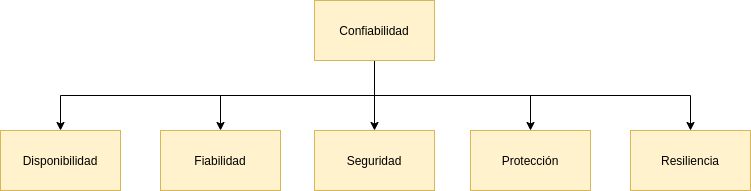
\includegraphics[width=\textwidth]{01-introduction/dependability.png}
  \caption{Principales aspectos de la confiabilidad}
  \label{fig:01-dependability}
\end{figure}

Para muchos sistemas de control, el tiempo es también un aspecto relevante a la
hora de garantizar su correcto funcionamiento. Estos son los llamados sistemas
de tiempo real. En un sistema normal, en el que se obtiene una salida al aplicar
una cierta lógica sobre la entrada, la corrección de dicha salida depende de la
corrección de la lógica aplicada, es decir, del cálculo realizado. No obstante,
cuando hablamos de sistemas de tiempo real, la corrección de la lógica no es
suficiente para determinar que el funcionamiento es correcto, sino que esta
corrección depende también del momento temporal en el que se obtiene
\cite{gambier_real-time_2004}. En otras palabras, si el cálculo es correcto pero
el resultado no llega en el momento en el que se necesita, se considera como un
fallo del sistema. Las tareas que ejecuta un sistema de tiempo real están, por
tanto, sujetas a restricciones temporales. Normalmente, hablamos de un tiempo
límite o \textit{deadline} antes del cuál se debe haber completado la tarea.
Comúnmente, se suelen clasificar las tareas en dos tipos dependiendo de las
consecuencias de incumplir con sus restricciones temporales:

\begin{itemize}
  \item Tareas de tiempo real «blandas»: Se denominan así aquellas tareas en las
        que no completar las mismas antes del límite supone una reducción en la
        calidad del servicio (QoS).
  \item Tareas de tiempo real «duras»: En estas tareas, el no cumplir con las
        restricciones temporales supone un fallo grave del sistema con posibles
        consecuencias catastróficas.
\end{itemize}

Para implementar estos sistemas, se hace uso de herramientas y algoritmos de
planificación de procesos específicos que permiten la ejecución de estos tipos
de tareas cumpliendo con sus restricciones temporales. Esto se explica en más
detalle en la sección \ref{sec:real-time}.

En este trabajo, nos centraremos especialmente en los sistemas de control
aplicados a entornos industriales. Debemos diferenciar entre dos conceptos: PCS
(\textit{Process Control System}), que es el sistema encargado de controlar una
parte concreta de la planta (p. ej., una turbina o un brazo robótico), e ICS
(\textit{Industrial Control System}), que se refiere al control de toda la
planta al completo. Un ICS está compuesto, por tanto, de múltiples PCS que se
encargan de controlar los distintos aspectos del proceso de producción. Estos
PCSs son sistemas empotrados como los que hemos comentado a los que se aplican
también los conceptos de confiabilidad y seguridad. En
\cite{krotofil_industrial_2013} se realiza un estudio del estado del arte en
cuanto a la seguridad de los ICS, concluyendo que, aunque las vulnerabilidades
de muchos de los sistemas actuales son conocidas, la aplicación de parches que
las solucionen son inviables debido a los altos costes asociados a la
recertificación o directamente debido a la incompatibilidad con algunos sistemas
más antiguos. Es necesario, por tanto, incorporar los conceptos de seguridad a
los procesos de diseño desde el primer momento para evitar dar lugar a estas
situaciones.

En 2007, Vestal \cite{vestal_preemptive_2007} publica una primera propuesta para
la planificación de conjuntos de tareas de criticalidad mixta. Este importante
avance es considerado por muchos como el inicio de la investigación en sistemas
de criticalidad mixta o MCS (\textit{Mixed-Criticality Systems}). La idea detrás
de estos sistemas es, como su propio nombre indica, poder ejecutar sobre una
misma plataforma hardware tanto tareas críticas como tareas no críticas o con
niveles de criticalidad menores, asegurando en todo momento que las
restricciones temporales se cumplen, al menos para las tareas más críticas.
Desde entonces, se han planteado muchos modelos para la implementación de estos
sistemas. En \cite{burns_mixed_2015}, Burns realiza una revisión de toda la
investigación realizada en este campo hasta marzo de 2019. Se muestran en esta
revisión algunas arquitecturas propuestas, además de las principales técnicas de
análisis para estos sistemas en plataformas uniprocesador y multiprocesador.
Burns identifica la conciliación entre la separación de los procesos y la
compartición de los recursos como el principal problema de los MCS. En este
aspecto, nuestro trabajo propone el uso de contenedores como medio de ejecución
de los distintos procesos sobre una misma plataforma consiguiendo esa
separación.

No podemos terminar nuestra revisión de los sistemas empotrados sin hablar sobre
el uso del kernel de Linux para su implementación. Como referencia, hemos tomado
dos estudios realizados en 2004 sobre el uso de Linux para sistemas empotrados
\cite{geer_survey_2004}\cite{henkel_munichmit_2004}. En el primero, se destaca
la buena situación de Linux en este campo, suponiendo las soluciones comerciales
basadas en el kernel de Linus Torvalds el 15,5\% del mercado. El segundo estudio
es una encuesta realizada a 268 personas que trabajan en el campo de los
sistemas empotrados, ya sea académicamente o de forma comercial. Lo más
destacable es que la mayoría de los participantes usan Linux en sistemas
empotrados para comunicaciones, dispositivos móviles o control de maquinaria.
Esto último es especialmente alentador para este trabajo, en el que pretendemos
usar Linux como base para la implementación de ICS.

\section{La nube en los sistemas industriales: fog/edge computing para sistemas
  de tiempo real}

Desde su aparición alrededor de 2006, la computación en la nube o \textit{cloud
  computing} ha experimentado un crecimiento abismal, cambiando completamente la
manera en la que las organizaciones gestionan su infraestructura y en la que los
usuarios acceden a servicios. Atendiendo a la definición del NIST
\cite{mell_nist_2011}, se trata de un modelo de prestación de servicios que
ofrece acceso ubicuo, prácticamente ilimitado y bajo demanda a un conjunto de
recursos de computación (p. ej., almacenamiento, tiempo de procesamiento,
comunicaciones), todo ello a través de internet. Sus principales características
son:

\begin{itemize}
  \item Acceso bajo demanda: El consumidor es el que decide qué recursos
        necesita y en qué cantidad, sin necesidad de intervención humana por parte del
        proveedor del servicio.
  \item Consumo a través de internet: El acceso a estos recursos se realiza
        mediante los protocolos ya conocidos y bien establecidos que potencian la web
        (p. ej., HTTP), permitiendo así un acceso ubicuo.
  \item Acceso compartido: Los recursos del proveedor se uniformizan, formando
        una especie de bolsa de recursos que es usada por múltiples consumidores
        (\textit{multi-tenant}). Por ejemplo, aunque desde el punto de vista de un
        usuario pueda parecer que tiene una CPU para él solo, en realidad la CPU
        física es usada por varios usuarios a la vez.
  \item Elasticidad: Dependiendo de la demanda, se pueden asignar o liberar los
        recursos de forma dinámica, consiguiente sistemas más eficientes y capaces de
        dar respuesta a cargas de trabajo más altas.
  \item Servicio medido: El uso de los recursos se monitoriza de forma
        automática, lo que proporciona transparencia tanto para el consumidor como el
        proveedor.
\end{itemize}

A raíz de la propuesta de la computación en la nube, han surgido varios modelos
de prestación de servicios a usuarios. Según el tipo de recurso que ofrecen,
estos modelos se pueden clasificar principalmente en SaaS (\textit{Software as
  a Service}), PaaS (\textit{Platform as a Service}) o IaaS
(\textit{Infrastructure as a Service}). Desde el punto de vista de los usuarios,
estos modelos tienen el beneficio de que permiten pagar solo por lo que
necesitas en cada momento, adaptándose perfectamente a tus necesidades. Además,
estos usuarios ya no se ven limitados por el hardware que poseen. Prácticamente
cualquier ordenador es capaz de conectarse a internet y, de esta forma, acceder
a unos recursos prácticamente ilimitados en la nube. Esto es especialmente
evidente para las empresas, las cuáles ya no necesitan mantener su propia
infraestructura de hardware para soportar su operación diaria, con los enormes
costes y complicaciones que esto supone.

En el campo del control industrial, en el que se centra este trabajo, podríamos
pensar en la nube como una plataforma ideal para procesar las enormes cantidades
de datos que producen las plantas e implementar las técnicas de aprendizaje
automático necesarias para mejorar su autonomía. No obstante, existe un gran
problema: la latencia. En el modelo de la nube, todo el procesamiento está
centralizado en un centro de datos\footnote{Normalmente, existen varios centros
  de datos distribuidos geográficamente, pero a efectos del problema que se
  plantea, se sigue viendo como una «centralización».}, el cuál se encuentra lejos
de la planta donde se recogen los datos. Enviar estos datos a la nube y esperar
una respuesta supone demasiado tiempo como para poder considerar delegar en ella
tareas de control de la operación de la planta. En entornos controlados, donde
el centro de datos se encuentra relativamente cerca de la planta, las pruebas
llevadas a cabo en \cite{hofer_industrial_2019} indican que la latencia puede
ser lo suficientemente predecible para la implementación de ciertos sistemas de
control con requisitos temporales suaves. Sin embargo, se trata de una situación
poco factible, ya que es inviable ubicar un centro de datos cerca de todas las
instalaciones industriales. En \cite{piggin_are_2015}, se analiza si los
ICS están preparados para ser desplazados a la nube, pero centrándose más en el
aspecto de la seguridad de estos sistemas. El autor identifica que, aunque la
nube es una plataforma muy robusta, también son flagrantes las dudas que produce
en cuanto a su seguridad frente a ataques. Por estas razones, no consideramos
que la nube sea un paradigma adecuado para dar respuesta a los nuevos requisitos
de la industria.

Aunque la nube no sea viable, bien es cierto que las ideas de elasticidad y
ubicuidad que plantea son interesantes para el problema en cuestión. Al final
del día, si queremos realizar análisis en tiempo real de los datos que generan
los procesos industriales para tomar decisiones, necesitamos más potencia
computacional de la que ningún dispositivo individual nos puede ofrecer. ¿La
solución? Aprovechar los recursos de computación de todos los dispositivos ya
presentes en las plantas industriales. De acercar estas ideas de la nube a los
dispositivos del borde de la red surgen dos nuevos paradigmas de computación:
\textit{fog} y \textit{edge computing}. En estos paradigmas, se pretende acercar
el procesamiento que se realiza sobre los datos a los propios dispositivos que
generan dichos datos. En el contexto industrial, esto también supone estar más
cerca de los dispositivos que deben actuar en respuesta a este procesamiento,
con lo que se obtendrían tiempos de respuesta mejores que con la nube. La
diferencia entre \textit{fog} y \textit{edge} radica en lo cerca del borde de la
red que ubiquemos el procesamiento de los datos, si bien es cierto que en
algunos escritos se usan los términos \textit{fog} y \textit{edge} de manera
intercambiable \cite{shi_edge_2019}, sin diferencia aparente entre ambos.

\begin{itemize}
  \item En \textit{fog}, se trata de nodos ubicados en la misma red local que
        las fuentes de datos.
  \item En \textit{edge}, los propios dispositivos que generan los datos ya
        realizan un cierto procesamiento de los mismos.
\end{itemize}

En la figura \ref{fig:02-cloud_fog_edge} se puede apreciar como estos dos
paradigmas, junto con la nube, constituyen una arquitectura por capas, donde
cada uno de ellos tiene unas características concretas. Se trata, por tanto, de
modelos complementarios, no exclusivos. En la capa \textit{edge}, donde se
generan los datos, se pueden implementar los mecanismos de control con
restricciones más duras, ya que se tienen unos tiempos de respuesta más rápidos
al actuar directamente en base a los datos generados. En la capa \textit{fog},
los nodos pueden realizar tareas de análisis de datos más exigentes, dado que
poseen más capacidad de computación que los dispositivos del \textit{edge}.
También se pueden implementar aquí tareas de control. Por último, la nube
recibiría todos los datos producidos por la planta, además de otras plantas que
también posea la organización, realizando la agregación y el análisis en
profundidad de los datos, obteniendo informes que puedan ayudar a los
supervisores en la identificación de fallos y la mejora del rendimiento.

\begin{figure}
  \centering
  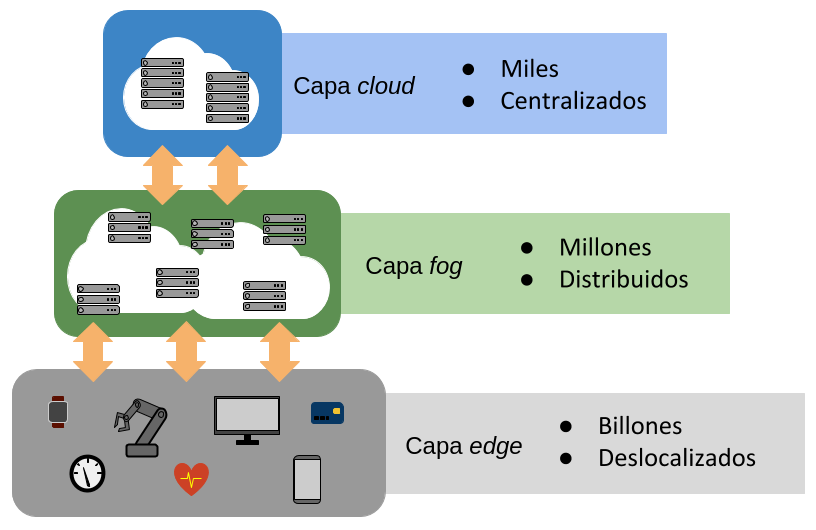
\includegraphics[width=0.7\textwidth]{02-state_of_the_art/cloud-fog-edge.png}
  \caption{Estructura por capas \textit{cloud-fog-edge}}
  \label{fig:02-cloud_fog_edge}
\end{figure}

Dejando atrás la ya explicada nube, vamos a adentrarnos más en el \textit{fog}.
Esta capa se compone de los llamados nodos \textit{fog}, que son los encargados
de llevar a cabo las distintas tareas. Cualquier dispositivo con capacidad de
procesamiento, memoria y conexión de red puede ser un nodo viable. De esta
forma, se pueden usar como nodos routers, switches y otros dispositivos de
redes, así como cámaras de videovigilancia. Se aprovecha la capacidad de
procesamiento de todos estos dispositivos cuando no se están usando al 100\%.
Como ya se ha indicado, estos nodos se encuentran ubicados en la misma red local
(LAN) que los dispositivos del borde de la red que generan los datos. Las
distintas tareas de análisis y control a realizar sobre estos datos se
distribuyen sobre los nodos \textit{fog} de forma dinámica dependiendo de la
carga de trabajo que posean los mismos. A la hora de asignar una tarea a un
nodo, siempre se debe intentar hacer de forma que el nodo elegido esté lo más
cerca posible de la fuente de los datos \cite{gedeon_fog_2018}. Esto es
especialmente importante para tareas de control, donde es posible que no todos
los nodos \textit{fog} de la planta tengan la latencia necesaria para cumplir
con los requisitos temporales. En este sentido, en \cite{pop_enabling_2018} se
propone el uso de TSN (\textit{Time-Sensitive Networking}) para las
comunicaciones en la capa \textit{fog}, con el objetivo de reducir estas
latencias. Este modelo de computación distribuida sobre una bolsa o
\textit{pool} de recursos es muy similar al que encontramos en la nube, con la
diferencia de que en el \textit{fog} estos recursos son mucho más limitados, por
lo que es también esencial optimizar el uso de los mismos. Debido a esta
similitud con el modelo de la nube, las mismas tecnologías de virtualización
usadas en ésta también son útiles en el nuevo paradigma \cite{yi_fog_2015}.
Algunos modelos ya han sido propuestos para la aplicación del \textit{fog} a los
sistemas industriales y el modelado de la Industria 4.0
\cite{verba_modeling_2019} \cite{tseng_lightweight_2018}.

Aunque la capacidad de procesamiento del \textit{fog} es mucho menor que la de
la nube, sigue siendo útil para realizar algunas tareas menos intensivas
evitando tener que desplazar todos los datos a la nube, con la latencia y la
carga en la red que eso supone. Como consecuencia del avance del IoT
(\textit{Internet of Things}) industrial, que es considerada una de las
tecnologías más importantes para la Industria 4.0 \cite{lu_industry_2017}, el
número de dispositivos presentes en las plantas y, por tanto, la cantidad de
datos que se generan va a ser mucho mayor, poniendo aún más presión sobre la
red, que es donde se podría producir el cuello de botella \cite{shi_edge_2016}.
El \textit{edge} trata de solucionar esto al reducir la cantidad de datos que se
deben enviar hacia las capas superiores procesando una parte de ellos de forma
local. Cabe destacar que el \textit{fog} también permite relajar el tráfico de
red \cite{wang_traffic_2019}. Los dispositivos del borde de la red, aún
ofreciendo menos potencia que la combinada del \textit{fog}, también pueden ser
usados para realizar algunas acciones sobre los datos. En concreto, las tareas
de control que requieran de un tiempo de respuesta más rápido pueden realizarse
en esta capa, tomando decisiones directamente sobre los datos que recoge el
dispositivo. Por otra parte, Khan \cite{khan_edge_2019} identifica la falta de
confianza en los sistemas \textit{edge} como uno de los principales problemas a
los que se enfrenta el paradigma, además de la integración de sistemas y la
movilidad. Esta falta de confianza es especialmente grave si pretendemos
desplegar sistemas de control críticos sobre plataformas de este tipo. Como
solución al problema de la confianza, Stanciu \cite{stanciu_blockchain_2017}
propone usar tecnología de \textit{blockchain} para desplegar sistemas de
control distribuidos en el \textit{edge}.

Sectores como el automovilístico, energético o de alimentación están muy
interesados en el desarrollo de la Industria 4.0 debido a los importantes
beneficios que se estima que puede tener para sus procesos. Gracias al 5G y a
las mejoras en las comunicaciones, el IoT se convierte en una idea capaz de dar
a las organizaciones una cantidad de información sobre sus procesos industriales
jamás vista antes. Estos datos son la base de la Industria 4.0
\cite{khan_perspective_2016}, ya que permiten la definición de sistemas
ciber-físicos y gemelos digitales que replican perfectamente los procesos
físicos en el plano digital, lo que abre la puerta a un control inédito sobre
dichos procesos. Además de las comunicaciones, otro reto muy importante para la
consecución de estos objetivos es el modelado de estos sistemas cuidando los
aspectos deseados de seguridad y fiabilidad \cite{farsi_industry_2019}. En este
sentido, creemos que el \textit{fog} es un modelo de computación que puede
facilitar el diseño de estos CPS al proporcionar una plataforma robusta y
unificada sobre la que implementarlos.

\section{Tecnologías de virtualización: hipervisores y contenedores}

De manera simple, la virtualización consiste en abstraer ciertas capas de un
sistema convencional (p. ej., el hardware). Sobre estas abstracciones se pueden
ejecutar procesos o sistemas completos de manera aislada. Este aspecto es el que
hace de la virtualización un concepto tan relevante para la computación en la
nube, ya que posibilita el acceso compartido a los recursos. Por ejemplo, sobre
una misma CPU se podrían ejecutar varios sistemas operativos completamente
funcionales de forma que ninguno de ellos sepa de la existencia de los otros.
Cada uno de estos sistemas cree que tiene una CPU completa para él gracias a la
abstracción del hardware. Aunque las tecnologías de virtualización han
experimentado un empuje enorme en los últimos años debido a la expansión de la
nube, no se trata de una idea novedosa. En 1974, Popek y Goldberg
\cite{popek_formal_1974} definían los requisitos que debía cumplir una
plataforma para poder virtualizar sistemas completos. Hoy en día, hablamos de
virtualización en dos niveles diferentes: a nivel del hardware (máquinas
virtuales) o a nivel del sistema operativo (contenedores).

Lo que se quiere decir con virtualización a nivel del hardware, es que es éste
el que se abstrae. Esto es precisamente lo que sucede con las máquinas
virtuales. El hardware «real» se puede fraccionar para asignarlo a las diversas
máquinas virtuales, que lo usan como si se tratase de una plataforma física
normal y corriente. Así, se puede regular la cantidad de CPU, memoria RAM o,
incluso, acceso a dispositivos de I/O que tiene cada máquina virtual. Todo esto
es posible gracias a los hipervisores, que son la pieza de software encargada de
abstraer el hardware y regular su uso por parte de las máquinas virtuales.
Dependiendo de la relación existente entre el hipervisor y el hardware que
abstraen, nos encontramos con hipervisores de tipo 1 y 2. Un hipervisor de tipo
2 se ejecuta sobre un sistema operativo tradicional, que recibe el nombre de
anfitrión, mientras que los de tipo 1 prescinden del anfitrión, ejecutándose
directamente sobre el hardware que gestionan (\textit{bare metal}). En la figura
\ref{fig:02-hypervisors} se representa gráficamente esta diferencia.

\begin{figure}
  \centering
  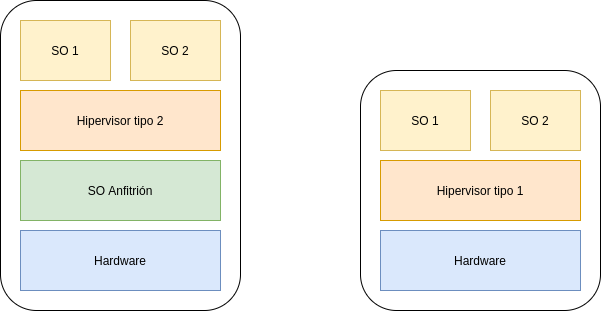
\includegraphics[width=0.8\textwidth]{02-state_of_the_art/hypervisors.png}
  \caption{Capas de la virtualización mediante hipervisores de tipo 1 y 2}
  \label{fig:02-hypervisors}
\end{figure}

Como es obvio, los hipervisores de tipo 1 suponen una solución mucho más liviana
que los de tipo 2 al no tener un anfitrión. Por otra parte, pueden asignar
prácticamente todos los recursos hardware de la plataforma a las máquinas
virtuales de forma dinámica, mientras que los de tipo 2 se ven restringidos a
los límites impuestos por el anfitrión. Los hipervisores de tipo 2 son más
utilizados en el ámbito personal, con herramientas como VirtualBox o VMWare
siendo muy utilizadas para la prueba de software, mientras que los de tipo 1 son
los que predominan a nivel empresarial e industrial, con claros ejemplos como
PikeOS o Xen. Este último supuso un importante avance en la ejecución segura y
aisla de máquinas virtuales sobre hardware de uso común \cite{barham_xen_2003}.
En lo que a sistemas de tiempo real se refiere, RT-Xen \cite{xi_rt-xen_2011} se
presentó como un marco de referencia para la planificación de procesos con
restricciones temporales en sistemas Linux virtualizados usando Xen, obteniendo
prometedores resultados.

Mientras que en la virtualización a nivel del hardware las máquinas virtuales
contienen un sistema operativo completo, en la virtualización a nivel del
software solo se virtualizan procesos. Estos procesos virtualizados, que reciben
comúnmente el nombre de contenedores, acceden a los servicios básicos del
sistema operativo anfitrión. De forma análoga a los hipervisores, los motores de
contenedores son los encargados de gestionar los procesos y su acceso al sistema
operativo que comparten. Realmente, los procesos contenerizados se ejecutan
sobre el sistema anfitrión como lo harían los procesos «nativos». La única
diferencia se encuentra en que los procesos contenerizados están aislados del
resto. Estos procesos solo pueden ver al resto de procesos de su mismo
contenedor, no los del resto de contenedores ni los no contenerizados. Para
conseguir este aislamiento, los motores de contenedores aprovechan varias
características del kernel de Linux, entre las que destacamos:

\begin{itemize}
  \item Espacios de nombres (\textit{namespaces}): los identificadores de
        proceso (PID), las interfaces de red o la parte del sistema de ficheros que
        puede ver un proceso contenerizado depende del espacio de nombres al que se
        asigne cuando se crea. Usando esta herramienta, se puede restringir lo que ven
        los contenedores del sistema anfitrión.
  \item Grupos de control (\textit{control groups}): Los \texttt{cgroups} son
        mecanismos que permiten regular el acceso al hardware por parte de los
        contenedores, así como su acceso compartido.
\end{itemize}

A primera vista, cabría pensar que, dado que contienen un sistema operativo
completo, las máquinas virtuales son mucho más pesadas que los contenedores. No
obstante, en trabajos como \cite{manco_my_2017} \cite{felter_updated_2015} se
desmiente esta percepción. Concretamente, en el último se compara el popular
motor de contenedores Docker con KVM, un famoso hipervisor para Linux, llegando
a la conclusión de que ninguno de los dos penaliza de manera significativa el
rendimiento en cuanto a uso de CPU o memoria, si bien es cierto que las máquinas
virtuales de KVM obtenían peores resultados en las operaciones de I/O. Por otro
lado, la seguridad en los contenedores es un aspecto todavía en desarrollo
\cite{randal_ideal_2020}, sobre todo en la seguridad del kernel compartido.

Existen múltiples motores de contenedores usados ampliamente en la actualidad,
como es el caso de Docker, Rocket (rkt) o LXC (\textit{LinuX Containers}).
Kozhirbayev y Sinnot \cite{kozhirbayev_performance_2017} realizaron en 2017 una
comparativa del rendimiento entre Docker y LXC\footnote{Concretamente, se hace
  uso de Flockport.}. Los resultados obtenidos coinciden con los vistos en
\cite{felter_updated_2015} en tanto que los procesos contenerizados no tienen
una penalización en el consumo de CPU o RAM frente a los nativos, aunque sí que
se observa esta penalización en las operaciones de I/O. Como el rendimiento es
similar para todos los motores de contendores, se ha decidido poner el foco
sobre Docker para este trabajo debido a que es el más popular, con el
consecuente impacto que esto tiene en la calidad del soporte y de la
documentación disponible.

\begin{figure}
  \centering
  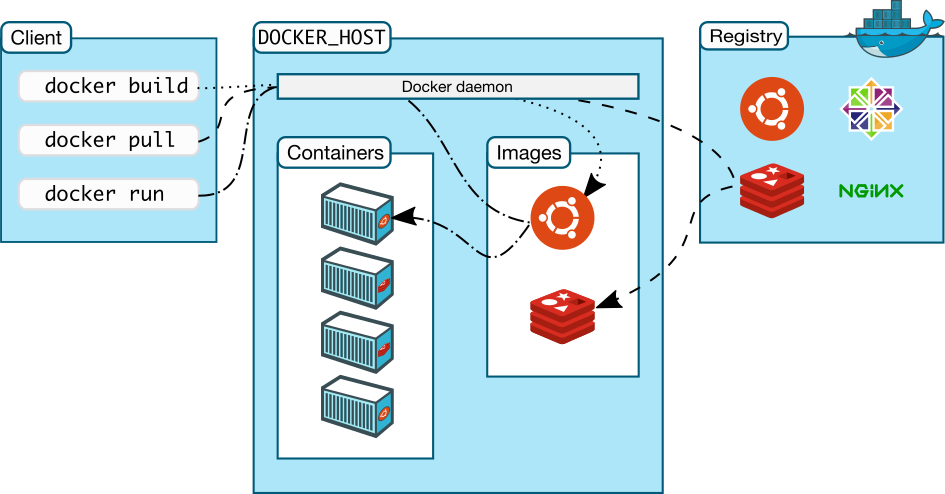
\includegraphics[width=\textwidth]{02-state_of_the_art/docker.png}
  \caption{Esquema de funcionamiento de Docker}
  \label{fig:02-docker}
\end{figure}

En Docker, al igual que en muchos otros motores de contenedores, los
contenedores se lanzan a partir de imágenes, definidas mediante un
\texttt{Dockerfile}. Una imagen es reutilizable y universal, pudiendo lanzar
réplicas de un mismo contenedor en cualquier plataforma soportada por la imagen.
Para trabajar con imágenes y contenedores, el sistema Docker se compone de dos
partes principales: el demonio\footnote{Un demonio o \textit{daemon} es un tipo
  de proceso que se ejecuta en segundo plano para ofrecer un servicio.} y el
cliente. El demonio es el encargado de realizar todas las soperacones
relacionadas con imágenes o contenedores, incluyendo su construcción,
lanzamiento y gestión posterior. Para realizar estas acciones, expone una API
con la que pueden interactuar los distintos clientes, siendo el oficial que
proporciona Docker una aplicación de línea de comandos. A estos dos componentes
se podría añadir un tercero, el registro de imágenes. Como su propio nombre
indica, se trata de una especie de base de datos de imágenes listas para su uso.
De esta forma, se pueden almacenar y compartir imágenes entre varios
dispositivos a través de la red. No obstante, se puede hacer uso de Docker de
manera local sin necesidad de usar un registro externo. Un esquema del
funcionamiento de Docker que se acaba de explicar se puede ver en la figura
\ref{fig:02-docker}.

Centrando nuestra atención de nuevo en los sistemas de control industrial, se
plantea la posibilidad de implementarlos usando contenedores
\cite{hofer_industrial_2019}, aunque los principales inconvenientes
identificados son los relacionados con la seguridad. En
\cite{cinque_rt-cases_2019}, los autores proponen un modelo de planificación de
procesos contenerizados para conjuntos de tareas con distintos niveles de
criticalidad, defendiendo el uso de contenedores por su capacidad de
aislamiento. Sin embargo, en la encuesta sobre contenerización para tiempo real
realizada por Struhár et al. en 2020 \cite{struhar_real-time_2020}, se llega a
la conclusión de que son necesarias mejores herramientas para la gestión de
contenedores de tiempo real. Por ello, en este trabajo se plantea el desarrollo
de una herramienta para este fin como prueba de concepto. Los autores del
estudio destacan también la falta de un mecanismo determinista de comunicación
entre procesos contenerizados y de herramientas de validación y prueba, además
de los problemas de seguridad ya mencionados.

\section{Aspectos de computación en tiempo real: RTOS, algoritmos de
  planificación y herramientas}
\label{sec:real-time}

En esta sección, se va a explicar con mayor detalle el funcionamiento de los
sistemas de tiempo real ya mencionados en las secciones anteriores. En estos
sistemas, el tiempo es un factor crucial a la hora de determinar la validez de
las salidas. De esta forma, las tareas ejecutadas se ven limitadas por
restricciones temporales. Dependiendo de la severidad de las consecuencias del
incumplimiento de las restricciones, solemos hablar de tareas y restricciones
duras o blandas. Las restricciones duras son aquellas que, si se incumplen,
tienen consecuencias son muy graves, como pueden ser daños a la vida de las
personas en el caso de sistemas que sean críticos. En cuanto a las restricciones
blandas, solo se experimenta una pérdida de calidad en el servicio cuando se
incumplen, aunque se suele limitar el número de incumplimientos permitido. En la
figura \ref{fig:02-deadlines} se muestra la diferencia entre los dos tipos de
restricciones según su función de utilidad \cite{wang_introduction_2013}, que es
la que define el valor de la salida del sistema en función del tiempo. Como se
puede apreciar, el resultado de una tarea dura solo es útil si se da entre el
inicio de la tarea y su límite temporal fijado, provocando daños de cualquier
otra manera. En las tareas blandas, el resultador puede tener valor incluso si
se obtiene después del límite, aunque se va reduciendo con el tiempo.

Debido a la gran responsabilidad que recae sobre el cumplimiento de estos
requisitos, los sistemas empotrados sobre los que se ejecutan estas tareas
tienen características diferentes a las de los sistemas de uso general. A nivel
del hardware, por ejemplo, las CPU tienen un diseño más simple que haga más
fácil verificar el determinismo en sus operaciones. En
\cite{rotenberg_chapter_2005}, Rotenberg y Anantaraman describen el
funcionamiento de las CPU de alto rendimiento y las comparan con las empotradas.
La ejecución predictiva, por ejemplo, es severamente limitada en los sistemas
empotrados. Por otro lado, las operaciones de acceso a caché y RAM suponen están
optimizadas para necesitar un menor número de ciclos. Normalmente, el conjunto
de instrucciones (ISA) de estas CPU es reducido, conocido como RISC, reduciendo
la complejidad y facilitando la programación a bajo nivel. ARM es una de las
arquitecturas de microprocesador basadas en RISC más usadas para el diseño de
sistemas empotrados. Otro aspecto diferencial es el número de núcleos o
\textit{cores} presentes en los procesadores. Poseer varios núcleos hace posible
la ejecución en paralelo de instrucciones, mejorando el rendimiento en los
sistemas. No obstante, este paralelismo dificulta asegurar el determinismo,
aunque algunos algoritmos de planificación de procesos han sido propuestos
\cite{anderson_edf-based_2005} y la investigación es activa en este área. Para
asegurar además que las tareas se puedan ejecutar correctamente, los sistemas de
tiempo real suelen dejar capacidad de CPU extra libre.

\begin{figure}
  \centering
  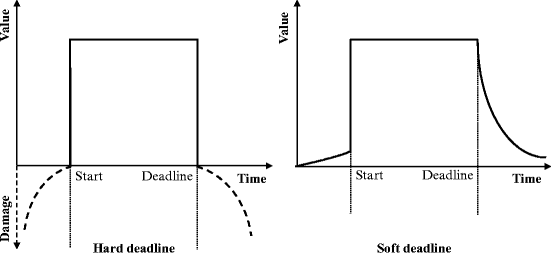
\includegraphics[width=0.8\textwidth]{02-state_of_the_art/deadlines.png}
  \caption{Funciones de utilidad para restricciones temporales duras y blandas}
  \label{fig:02-deadlines}
\end{figure}

Además del hardware, el software usado para implementar estos sistemas también
es especial. Los lenguajes y herramientas deben proporcionar al programador
ciertas comodidades para la implementación de procesos en tiempo real
\cite{burns_real-time_2009}:

\begin{itemize}
  \item Especificar momentos en los que las acciones se deben realizar.
  \item Especificar los momentos antes de los cuales las acciones deben terminar.
  \item Permitir la ejecución repetitiva (periódica y aperiódica) de trabajo.
  \item Limitar la varianza en las operaciones de entrada y salida.
  \item Responder a situaciones donde no todas las restricciones temporales se
        pueden cumplir.
  \item Responder a situaciones en las que los requisitos de tiempo cambian de
        manera dinámica.
\end{itemize}

Una parte muy importante de los sistemas empotrados es su sistema operativo, el
cual gestiona los recursos físicos de la plataforma y controla el uso de los
mismos por parte de los procesos implementados por los desarrolladores. Al igual
que ocurre con el hardware, estos sistemas operativos también tienen
características diferentes a los de propósito general para poder dar cobijo a
tareas con restricciones temporales, recibiendo el nombre de RTOS (\textit{Real
  Time Operating System}). La principal diferencia, podríamos decir que se
encuentra en los algoritmos de planificación de tareas usados, aunque cabe
destacar que también hay otras áreas importantes como el acceso a memoria o la
gestión de las interrupciones. El algoritmo de planificación es, a grandes
rasgos, la política que decide en qué orden se ejecutan las tareas del sistema.
En los sistemas normales, normalmente se asigna a cada proceso una fracción
igualitaria de tiempo de CPU, ejecutándose hasta que consume su fracción de
tiempo o se bloquea (p. ej., por una operación de lectura o escritura). En los
sistemas de tiempo real, este método no es factible, ya que los procesos tienen
distintas prioridades y no pueden quedar a la espera de que otro proceso de
menor prioridad libere la CPU. Por ello, la planificación de procesos de tiempo
real es apropiativa (\textit{preemptive scheduling}), de forma que el sistema
operativo puede quitar la CPU a un proceso que está en ejecución para
asignársela a otro más prioritario. Como se destaca en
\cite{burns_scheduling_1991}, la planificación de procesos óptima para un
sistema de tiempo real «duro» depende enormemente del problema en cuestión. ¿Se
trata de un sistema uniprocesador o multiprocesador? ¿Todas las situaciones son
conocidas de antemano? ¿Las tareas son periódicas o aperiódicas? Dependiendo de
la situación, podemos encontrarnos con que un algoritmo de planificación es más
eficaz que otro.

Antes de entrar a explicar algunos de los algoritmos de planificación de tareas
más importantes, debemos entender mejor como son estas tareas. Las tareas en un
sistema de tiempo real pueden ser provocadas por tiempo o por eventos. Las
tareas provocadas por tiempo son tareas periódicas, con un tiempo definido para
sus ciclos. Las caracterizamos con los siguientes atributos:

\begin{itemize}
  \item Tiempo de ejecución $WCET$ (\textit{Worst Case Execution Time}): Se trata
        del tiempo que se necesita para completar la tarea en el peor caso.
  \item Límite de tiempo $D$ (\textit{Deadline}): Momento temporal posterior a
        la activación de la tarea y antes del cuál se debe haber completado.
  \item Período $T$ (\textit{Period}): Es el tiempo que transcurre entre
        activaciones.
\end{itemize}

Estas tareas son ejecutadas por un reloj interno del sistema, el cuál debe ser
lo suficientemente preciso como para asegurar que los ciclos se cumplen. Por
otra parte, las tareas también pueden ser aperiódicas si son activadas por un
evento externo (p. ej., un cambio en el entorno, como sucede en algunos sistemas
de control) mediante mecanismos como las interrupciones. Las tareas aperiódicas
siguen teniendo $WCET$ y $D$, pero no tienen período $T$. En algunos casos,
existe un tiempo mínimo entre activaciones $T$, considerándose la tarea como
esporádica. En ocasiones, los sistemas empotrados limitan su arquitectura para
que solo haya tareas activadas por tiempo, evitando las interacciones y
comprobando de forma periódica si se ha producido un evento. De todos estos
atributos, el tiempo de ejecución en el peor caso es el más difícil de
determinar. Se trata de un límite superior que puede ser estimado usando métodos
estáticos, probabilísticos o, incluso, basados en mediciones. No obstante, la
fiabilidad de muchos de estos métodos se apoya en supuestos sobre el sistema y
su funcionamiento \cite{abella_wcet_2015}.

Para evaluar la efectividad de un algoritmo de planificación, solemos basarnos
en su capacidad para cumplir con todas las restricciones temporales de un
conjunto de tareas dado. Cuando se consiguen respetar todas estas restricciones,
se dice que la planificación (o el conjunto de tareas) es viable, mientras que
si el sistema se salta alguna, se suele decir que está sobrecargado. Un concepto
muy importante en el que se apoyan los algoritmos de planificación para
determinar la viabilidad de un conjunto de tareas es la utilización total de CPU
para dicho conjunto, definida como

\begin{equation}
  U = \sum_{i=1}^{n} \frac{C_{i}}{min(D_{i}, T_{i})}
\end{equation}

por Liu y Layland \cite{liu_scheduling_1973}, donde $C_{i}$, $D_{i}$ y $T_{i}$
son el tiempo de ejecución, límite temporal y período para la tarea $i$ del
conjunto, respectivamente.

Anteriormente, se ha indicado que la planificación de procesos de tiempo real es
apropiativa, de forma que el sistema operativo puede retirarle a un proceso los
recursos que tenía asignado para dárselos a otro de mayor prioridad. La
asignación de estas prioridades a las distintas tareas es la base de los
algoritmos de planificación. Estos algoritmos pueden ser de dos tipos: estáticos
o dinámicos. Los algoritmos estáticos realizan la planificación y asignan las
prioridades a las tareas antes incluso de tener que poner en marcha el sistema,
de forma \textit{offline}, ejecutándose luego las tareas en el orden determinado
por las prioridades establecidas. También conocida como planificación de
prioridades fijas FPS (\textit{Fixed-Priority Scheduling})
\cite{tilborg_fixed_1991}, para aplicar estos algoritmos es necesario conocer
todas las características del problema de planificación (número de tareas y sus
atributos) de antemano, lo cuál es imposible en algunas situaciones en las que
se desconoce la carga de trabajo futura del sistema. Uno de los algoritmos
estáticos más conocidos es RMS (\textit{Rate Monotonic Scheduling})
\cite{liu_scheduling_1973}\cite{kao_rate-monotonic_2008}, cuya idea principal es
que las tareas con los períodos más pequeños tienen mayor prioridad. En la
propuesta original de RMS realizada por Liu y Layland, asumen un conjunto de
tareas periódicas con $D=T$ y determinan el límite superior para la utilización
como

\begin{equation}
  U \leq n(2^{\frac{1}{n}} - 1)
\end{equation}

Esto implica que, para conjuntos de tareas muy grandes ($n \rightarrow \infty$),
la utilización de CPU tiene que ser inferior al 70\%, que es una cifra
relativamente baja. No obstante, si se cumplen todas estas condiciones, RMS
garantiza encontrar una planificación viable si es que existe, o lo que es lo
mismo, es un algoritmo óptimo. Otro problema de RMS es que requiere que el
período sea igual al límite de tiempo para cada tarea. Para solucionar este
problema, se propone DMT (\textit{Deadline Monotonic Scheduling})
\cite{audsley_hard_1991}, en el que los procesos se caracterizan con $C_{i} \leq
  D_{i} \leq T_{i}$.

Como ya se ha comentado, el principal problema de la planificación estática es
que se trata de algoritmos clarividentes, es decir, necesitan conocer toda la
información sobre el conjunto de tareas para poder determinar su viabilidad. Los
algoritmos dinámicos, por otra parte, permiten determinar esta viabilidad
en tiempo de ejecución, cambiando las prioridades de las tareas sobre la marcha
u \textit{online}. Uno de los algoritmos dinámicos más conocidos es EDF
(\textit{Earliest Deadline First}) \cite{liu_scheduling_1973}, donde las tareas
con menor tiempo restante antes de su límite temporal son las que reciben una
mayor prioridad. En este caso, el algoritmo es óptimo para conjuntos de tareas
donde se cumpla la condición \cite{zhang_schedulability_2009}

\begin{equation}
  U \leq 1
\end{equation}

No obstante, esta situación se da solo en los sistemas uniprocesador. En los
multiprocesador, determinar que la utilización es inferior al número de CPU no
es una condición suficiente para garantizar que el conjunto de tareas tenga una
planificación viable. En 2005, Anderson adapta EDF para sistemas multiprocesador
\cite{anderson_edf-based_2005}, consiguiendo una condición suficiente para
tareas de tiempo real blandas. Un enfoque diferente al de EDF lo proporciona MUF
(\textit{Maximum Urgency First}) \cite{stewart_real-time_1991}. En este
algoritmo, se trabaja en torno a la urgencia de cada tarea, que es determinada
según la combinación de varias prioridades. En concreto, cada tarea posee 2
prioridades fijas definidas antes de la ejecución y una dinámica, que se calcula
sobre la marcha, existiendo una relación de precedencia entre estas prioridades.

En el caso de ser necesario trabajar con tareas aperiódicas o esporádicas, se
puede aplicar alguno de los algoritmos propuestos en
\cite{sprunt_scheduling_1989}, entre los que destacamos DSA (\textit{Deferrable
  Server Algorithm}) y SSA (\textit{Sporadic Server Algorithm}).

Para terminar con el repaso de la computación de tiempo real, vamos a hacer un
breve repaso de algunos de los RTOS más utilizados. En
\cite{hambarde_survey_2014}, Hambarde realiza una comparación entre Windows CE,
VxWorks, QNX Neutrino y RTAI. El último, que es esencialmente una extensión del
kernel de Linux o co-kernel que da soporte a este tipo de cargas de trabajo,
obtiene los mejores resultados en latencia, \textit{jitter} y tiempo de
respuesta de entre los cuatro, si bien es cierto que su latencia ante
interrupciones es mayor que la de VxWorks. Además de RTAI, otros co-kernels para
Linux serían RTLinux y Xenomai. Todos estos co-kernels funcionan de manera
similar: implementan un despachador de interrupciones que captura las
interrupciones provenientes del hardware para redirigirlas a los procesos (tanto
normales como de tiempo real), mientras que también poseen un planificador de
procesos para asegurar que se cumplen las prioridades.

Además de los co-kernels, otra solución alternativa para Linux la encontramos en
el parche \texttt{PREEMPT\_RT}. El desarrollo de este parche es llevado a cabo
por programadores del kernel dentro de la fundación Linux y en paralelo con el
del propio kernel, lo que le da un cierto aire de «oficialidad». En esencia, los
cambios que aplica este parche sobre el kernel habilitan la planificación
apropiativa y aumentan el determinismo de ciertas operaciones. Este
acercamiento, al trabajar sobre un único kernel en vez de los dos que se
obtienen con las soluciones basadas en co-kernels, resulta en una mayor
facilidad a la hora de implementar procesos de tiempo real, ya que se realiza de
manera idéntica a los normales. Los co-kernels exponen interfaces especiales que
se salen de la interfaz estándar de Linux y con las que sus procesos deben
trabajar, algo que no ocurre con el parche \texttt{PREEMPT\_RT} y que hace que
sea muy fácil adaptar un proceso existente para que tenga un comportamiento más
determinista. Este parche habilita varios modos de planificación de procesos
nuevos para el planificador del kernel, entre los que destacaremos
\texttt{SCHED\_DEADLINE} \cite{noauthor_deadline_nodate}. Esta política de
planificación aplica el algoritmo EDF junto con CBS (\textit{Constant Bandwith
  Server}). El algoritmo CBS se encarga de asignar un ancho de banda a cada tarea,
de forma que una tarea concreta no pueda ejecutarse durante un tiempo superior a
su tiempo de ejecución dentro de cada período. De esta forma, se consigue el
aislamiento temporal de las tareas, evitando que el comportamiento de una de
ellas afecte a las demás. En cuanto a su rendimiento, el estudio llevado a cabo
en \cite{reghenzani_real-time_2019} determina que no es una solución apta para
sistemas de tiempo real duro, pero puede ser perfectamente usado cuando las
restricciones son más livianas. En cualquier caso, el rendimiento va a depender
enormemente del hardware utilizado y de la implementación de los drivers para
dicho hardware.

Para este trabajo, se ha decidido usar como plataforma objetivo
el sistema GNU/Linux parcheado con \texttt{PREEMPT\_RT} debido a que se adhiere
a la interfaz estándar del kernel y las tecnologías de virtualización mediante
contenedores presentes en la plataforma son muy maduras. El hecho de que no sea
un RTOS aceptable para sistemas con restricciones temporales duras nos es
indiferente para el alcance de este proyecto, dado que solo se busca implementar
una herramienta que sirva como prueba de concepto de las ideas planteadas.

\appendix
\pdfbookmark[-1]{Apéndices}{appendix}
\chapter{Estimación de costes del proyecto}

Al tratarse, mayoritariamente, de un proyecto de Ingeniería del Software, se ha
realizado también una estimación de los costes asociados a la realización del
mismo. Para ello, se ha aplicado un modelo basado en tiempo y materiales. En
2019, el coste salarial medio de un ingeniero informático recién salido de la
universidad en España era de entre 24.000 y 28.500 euros brutos al año. En esta
estimación, se ha asumido un salario mensual de 2.000€ brutos al mes, que es
aproximadamente un salario anual de 24.000€. Las tareas de coordinación y
dirección del jefe del proyecto se estiman en un 10\% del trabajo de ingeniería,
con un coste medio mensual de unos 5.000€ al mes para un ingeniero sénior.
Además, se ha supuesto también una jornada laboral que llega al máximo en España
de 40 horas semanales. También se tiene en cuenta el coste del hardware usado
para pruebas. La estimación final del coste de desarrollo de este proyecto se
muestra en la tabla \ref{tab:A1-costs}.

\begin{table}[H]
    \centering
    \begin{tabular}{ | >{\columncolor[gray]{0.8}}l | p{0.2\textwidth} r | }
        \hline
        Raspberry Pi 4B 4GB         &  & 60,00€     \\
        \hline
        Cable Ethernet              &  & 7,00€      \\
        \hline
        Cable de alimentación USB-C &  & 7,00€      \\
        \hline
        Mano de obra ingeniero      &  & 8.000,00€  \\
        \hline
        Mano de obra ingeniero jefe &  & 20.000,00€ \\
        \hline
        \multicolumn{1}{ r |}{}     &  & 28.074,00€ \\
        \cline{2-3}
    \end{tabular}
    \caption{Desglose de costes del proyecto}
    \label{tab:A1-costs}
\end{table}

A todo esto habría que sumarle el coste de la estación de trabajo usada para el
desarrollo del proyecto, la cuál consiste de un ordenador de sobremesa o
portátil y los periféricos necesarios, junto con los gastos asociados al consumo
eléctrico y el acceso a internet. Estos gastos se han omitido de la estimación
realizada debido a que son muy variables y tampoco tienen un impacto muy
representativo en los costes del proyecto.


\backmatter
\bibliographystyle{ieeetr}
\bibliography{sources}

\end{document}